
\chapter{Target tracking}
Target tracking plays a pivotal role in radar systems, where the primary objective is to estimate the trajectory,
position and other
characteristics of moving objects within a surveillance area. Derived from the foundational principles of the Kalman filter, target tracking algorithms are tailored to the specific requirements and challenges inherent in radar applications.

Radar-based target tracking encounters various complexities, including survivability and the presence of
multiple targets in the same neighbour. Survivability concerns the algorithm's ability to maintain
accurate estimates despite target maneuvers, occlusions, or potential target loss. Furthermore, the phenomenon of
multiple targets in the same neighbour introduces significant ambiguities and challenges in trajectory estimation and
association.

In the realm of single-target tracking, algorithms such as the Probabilistic Data Association (PDA) filter and its derivatives, such as the Joint Probabilistic Data Association (JPDA) filter or the Integrated Probabilistic Data Association (IPDA) filter, are commonly employed. These algorithms provide robust solutions for associating measurements with existing tracks and updating target state estimates in dynamic scenarios.

Beyond single-target tracking, radar systems often necessitate multi-target tracking approaches. These approaches,
particularly those based on Random Finite Sets (RFS), offer advanced capabilities for tracking multiple targets simultaneously. RFS-based filters, including the Probability Hypothesis Density (PHD) filter and the Multi-Bernoulli filter, excel in scenarios where the number of targets is uncertain or dynamic.

In this chapter, we delve into the intricacies of radar-based target tracking algorithms, exploring their theoretical foundations, practical implementations, and performance characteristics. By understanding the diverse range of tracking algorithms available and their respective strengths, we can design and deploy effective tracking systems to meet the demands of modern surveillance and reconnaissance applications.

\section{Data association}
\label{sec:data_association}
Data association uncertainty arises in remote sensing systems, such as radar, sonar, or electro-optical devices, when
measurements are obtained from sources that may not necessarily be the target of interest \cite{BarShalomPDA}. This uncertainty
occurs particularly in situations where the target signal is weak, necessitating a lower detection threshold, which may result in the detection of background signals, sensor noise or clutter. Additionally, data association uncertainty can occur when multiple targets are present in close proximity. Utilizing spurious measurements in a tracking filter can lead to divergence of the estimation error and, consequently, track loss.

Addressing this challenge involves two primary problems. The first is the selection of appropriate measurements to
update the state of the target of interest in the tracking filter, which can be a Kalman filter or an extended Kalman
filter. The second problem involves determining whether the filter needs modifications to account for data
association uncertainty. The objective is to obtain the minimum mean square error (MMSE) estimate of the target state
and associated uncertainty.

The optimal estimator involves the recursive computation of the conditional probability density function (pdf) of the
state, with detailed conditions provided under which this pdf serves as a sufficient statistic in the presence of
data association uncertainty.
  \subsection{Validation region}
    \label{sec:validation_region}
In target tracking scenarios, the process of signal detection provides measurements, from which the appropriate ones
for inclusion in the target state estimator are chosen. In radar systems, for instance, the signal reflected from the
target of interest is sought within a specific time interval, determined by the expected range of the target when it
reflects the transmitted energy. A range gate is established, and detections falling within this gate can be
associated with the target of interest. These measurements could include informations such as range, azimuth, elevation,
or direction cosines. For radar or active sonar, we might also measure how fast something is moving toward or away
from us. For passive sonar, we might look at the direction something's coming from, when it arrives, and the
difference in sounds it makes. And for optical sensors, we might measure the angle it is seen from. By setting up a
multidimensional gate, the signal from the target is detected efficiently, avoiding the need to search for it across the entire measurement space.

However, while a measurement within the gate is a candidate for association with the target, it is not guaranteed to
have originated from the target itself. Thus, the establishment of a validation region becomes necessary. The
validation region is designed to ensure that the target measurement falls within it with a high probability, known as
the gate probability, based on the statistical characterization of the predicted measurement. In the event, where more
than one detection appears within the gate, association uncertainty arises. With this uncertainty, it is important to
figure out which measurement really comes from the target and should be used to update our tracking information. This includes things like the target's estimated position and its variability, or more broadly, the key information we need about the target. Measurements outside the validation region can be disregarded, as they are too distant from the predicted measurement and are unlikely to have originated from the target of interest. This scenario typically arises when the gate probability is close to unity, and the statistical model used to define the gate is accurate.
\section{Clutter}
When it comes to clutter, two scenarios may occur. The first one is a single target in clutter. This problem of
tracking a single target in clutter appears when several measurements appear in the validation region. The
validated measurements comprise the accurate measurement, if detected within this region, along with spurious
measurements originating from clutter or false alarms. In air traffic control systems, where cooperative targets are
involved, each measurement includes a target identifier known as the squawk number. If this identifier is entirely
reliable, data association uncertainty is eliminated. However, in cases where a potentially hostile target is non-cooperative, data association uncertainty becomes a significant challenge.

Figure \ref{fig:singleTargetInClutter} illustrates a scenario involving multiple validated measurements. The validation region depicted in the
figure is two-dimensional and takes the form of an ellipse centered at the predicted measurement $\hat{z}$. The
elliptical shape of the validation region arises from the assumption that the error in the target's predicted
measurement, known as the innovation, follows a Gaussian distribution. The parameters defining the ellipse are
determined by the covariance matrix $S$ of the innovation.

All measurements within the validation region have the potential to originate from the target of interest, although
only one of them is the true measurement. As a result, the possible association events include: $z_1$ originating
from the target, with $z_2$ and $z_3$ being from clutter; $z_2$ originating from the target, with $z_1$ and $z_3$
being from clutter; $z_3$ originating from the target, with $z_2$ and $z_1$ being from clutter; or all measurements
being from clutter. These association events are mutually exclusive and exhaustive, enabling the application of the
total probability theorem to obtain the state estimate in the presence of data association uncertainty.

Under the assumption of a single target, the spurious measurements are considered random interference. A common model for such false measurements assumes that they are uniformly spatially distributed and independent across time, corresponding to residual clutter. Any constant clutter is assumed to have already been removed.

\begin{figure}[h]
  \centering
  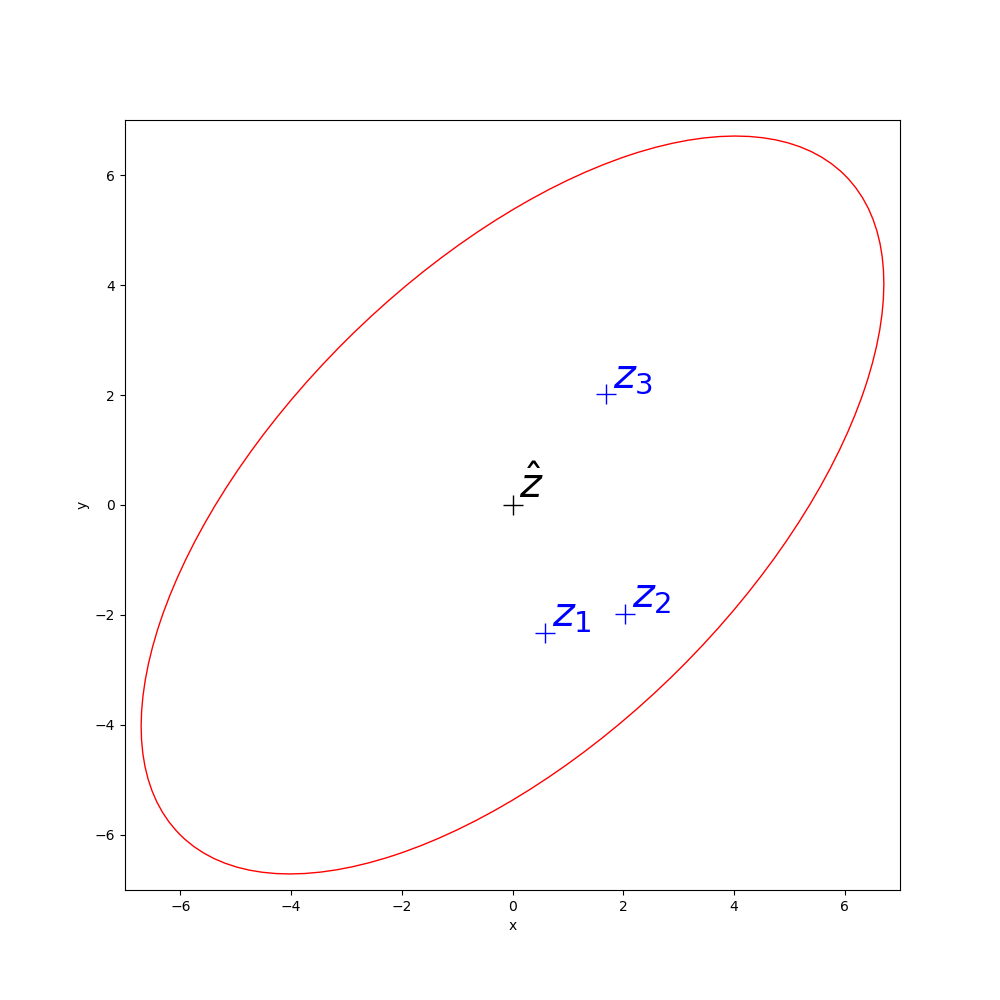
\includegraphics[width=10cm]{text/chapter_02/imgs/clutter_singleTarget}
  \caption{Several measurements $z_i$ appeared in the validation region of a single target. $\hat{z}$ is a predicted
  measurement and none or any of the measurement $z_1 - z_3$ may have originated from the target.}
  \label{fig:singleTargetInClutter}
\end{figure}

When several targets as well as clutter or false alarms appear in the same neighbour, the data association becomes
even more challenging. Figure \ref{fig:twoTargetsInClutter} shows this scenario, where predicted measurement for the
targets are close to each other. These predicted points are labeled as $\hat{z_1}$ and $\hat{z_2}$. In this figure
many association combinations are possible; $z_1$ from target $\hat{z_1}$ or clutter; $z_2$ from target $\hat{z_1}$
or clutter; $z_4$ from target $\hat{z_2}$ or clutter; $z_3$ from target $\hat{z_1}$ or target $\hat{z_2}$ or clutter. However, if $z_3$ originated from target $\hat{z_1}$, then it is probable, that $z_4$ originated from target $\hat{
    z_2}$.

This scenario demonstrates the intricate relationships among associations when persistent interference from neighboring targets coexists with random interference or clutter. In such cases, joint association events become necessary to properly account for these dependencies.

A more complex scenario may arise due to the inherent finite resolution capability of signal processing systems. While each measurement is typically assumed to originate from either a target or clutter, an additional possibility must be considered: the merging of detections from multiple targets. Specifically, measurement $z_3$ could potentially result from such merging, representing an unresolved measurement. This introduces a fourth origin hypothesis for a measurement lying within the intersection of two validation regions.

The discussion highlights the challenges associated with associating measurements to tracks. The complete problem
involves associating measurements at each time step, updating the track's sufficient statistic, and propagating it to
the subsequent time step.

\begin{figure}[h]
    \centering
    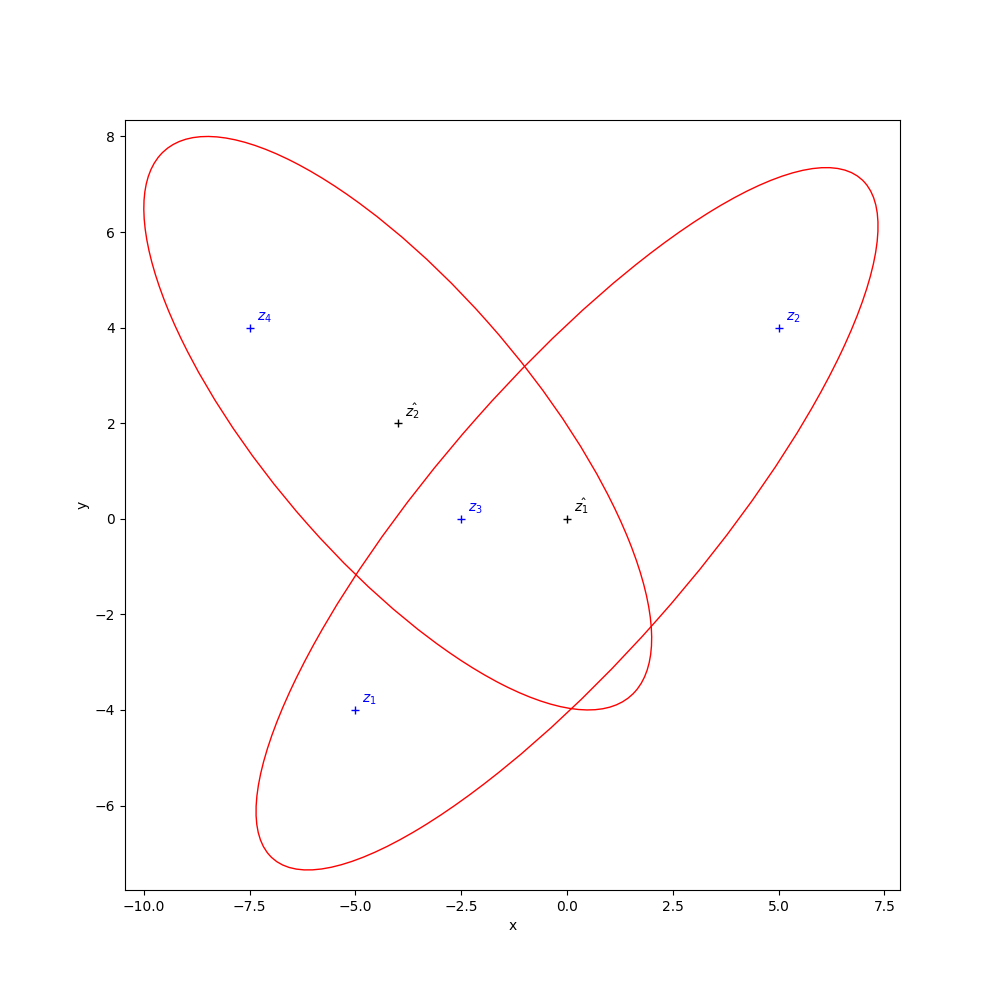
\includegraphics[width=10cm]{text/chapter_02/imgs/clutter_multiTarget}
    \caption{Several measurements $z_i$ appeared in the validation region of one of targets $\hat{z_1}$ or $\hat{z_2}$. $\hat{z_1}$ and $\hat{z_2}$ are predicted
    measurements and none or any of the measurement $z_1 - z_3$ may have originated from the target $\hat{z_1}$ and none or any of the measurement $z_3 - z_4$ may have originated from the target $\hat{z_2}$.}
    \label{fig:twoTargetsInClutter}
\end{figure}


\section{Single target tracking}
Single Target Tracking algorithms are specifically designed to track a single target in presence of clutter and other
sources
of interference. Unlike conventional Kalman filters, which is not inherently equipped to handle clutter. Single Target
Tracking algorithms incorporate mechanisms to enhance target survivability in cluttered environments.

One prominent algorithm in the data association category of target tracking is the Probabilistic Data Association filter. The PDA filter addresses the challenge of associating measurements with the correct target while accounting for data association uncertainty. This uncertainty arises from the presence of clutter and the possibility of spurious measurements.


\subsection{PDA filter}
\label{sec:pda_filter}
The Probabilistic Data Association algorithm computes the association probabilities for each validated measurement at
the current time with respect to the target being tracked. This probabilistic or Bayesian information serves as a
foundation for the Probabilistic Data Association Filter tracking algorithm, which effectively addresses the uncertainty regarding the origin of measurements. In scenarios where the state and measurement equations are linear, the resulting PDAF algorithm operates based on the Kalman Filter. However, if the state or measurement equations are non-linear, the PDAF algorithm is instead based on the Extended Kalman Filter. This adaptation allows the PDAF algorithm to accommodate non-linearity in the system dynamics or measurement processes, ensuring robust performance in diverse tracking scenarios.

The PDAF algorithm comes with many assumptions:
\begin{enumerate}
    \item Only one target of interest is present, whose state $x \in R^{n_x}$ is assumed to evolve in time according to the equation
        \begin{align}
            x_k &= F_{k-1} x_{k-1} + w_{k-1},
        \end{align}
        with the true measurement $z_k \in R^{n_z}$ given by
        \begin{align}
            \label{eq:pda_A1_eq2}
            z_k &= H_k x_k + v_k,
        \end{align}
        where $w_{k-1}$ and $v_k$ are zero mean mutually independent, white Gaussian noise variables with covariances $Q_{k-1}$ and $R_k$, respectively.
    \item The track has been initialized.
    \item The past information through time $k-1$ about the target is summarized approximately by a suffifient statistic in the form of the Gaussian posterior
        \begin{align}
            p(x_{k-1}|z_{k-1}) &= \mathcal{N}(x_{k-1}; x_{k-1|k-1}, P_{k-1|k-1})). \label{eq:pda_A3}
        \end{align}
    \item At each time a measurement validation region is set up around the predicted measurement to select the candidate measurements for association to the target of interest.
    \item If the target was detected and the corresponding
    measurement fell into the validation region, then,
    according to \eqref{eq:pda_A1_eq2}, at most one of the validated measurements can be target originated.
    \item The remaining measurements are assumed to be due
    to false alarms or clutter and are modeled as independent and identically distributed with uniform spatial distribution, and the number of false alarms or clutter points obeys either a Poisson distribution, that is, a spatial Poisson process, with known
    spatial density $\lambda$, or a diffuse prior.
    \item The target detections occur independently over time
    with known probability $p_D$.
\end{enumerate}
All these assumptions make a filter for state estimation, that is almost as simple as Kalman filter, but more effective in the presence of clutter.

As well as the Kalman Filter, the PDAF also consists of prediction and update step. Before the update step, two
additional steps occur -- measurement validation and data association.
 \subsubsection{PDAF predict step}
The prediction step of PDA filter from time $k-1$ to $k$ is as in the standard KF,
\begin{align}
    x_{k|k-1} &= F_{k-1}x_{k-1|k-1},\\
    \eta_{k|k-1} &= H_k x_{k|k-1},\\
    P_{k|k-1} &= F_{k-1} P_{k-1|k-1} F_{k-1}^T + Q_{k-1},
\end{align}
where $P_{k-1|k-1}$ is from the equation \eqref{eq:pda_A3}. The innovation covariance matrix $S_k$ is computed as
\begin{align}
    S_k &= H_{k} P_{k|k-1} H_{k}^T + R_{k}. \label{eq:pda_S}
\end{align}

\subsubsection{PDAF measurement validation step}
As discussed in Section \ref{sec:validation_region}, measurements considered to be originated from a given target
should fall into validation region. This elliptical region is formulated as
\begin{align}
    \nu(k,\gamma) &= \bigcup_{z \in Z_k}[(z - \hat{z}_{k|k-1})^T S_k^{-1} (z - \hat{z}_{k|k-1})) \leq \gamma], \label {eq:validation_region}
\end{align}
where $Z_k$ are all measurements at time $k$, $\gamma$ is the gate threshold corresponding to the gate probability $p_G$, which is the probability, that the region contains the correct measurement if detected and $S_k$ given in \eqref{eq:pda_S} is the covariance of the innovation.

\subsubsection{PDAF data association step}
The clutter in target tracking is assumed to be Poisson model with spatial density $\lambda$. In PDAF it yields to the association probability for $z_{i,k}$ being the correct measurement as

\vspace{-0.5cm}

\begin{align}
    \beta_{i,k} &=
    \begingroup
    \Large
    \begin{cases}
        \frac{\mathcal{L}_{i,k}}{1-p_D p_G + \sum_{j=1}^{m_k}\mathcal{L}_{j,k}}, & i=1, \dots, m_k, \\
        \frac{1-p_D p_G}{1-p_D P_G + \sum_{j=1}^{m_k}\mathcal{L}_{j,k}}, & i =0,
    \end{cases}
    \label{eq:pda_beta}
    \endgroup
\end{align}
where $i=0$ means none is correct, $p_D$ is the detection probability, $p_G$ is the gate probability analogous to \eqref{eq:validation_region}, and
\begin{align}
    \mathcal{L}_{i,k} &= \frac{\mathcal{N}(z_{i,k};\hat{z}_{k|k-1}, S_k) p_D}{\lambda} \label{eq:pda_likelihood}
\end{align}
is the likelihood ratio of the measurement $z_{i,k}$ from the validation region. The parameter $\lambda$ (the density
of the spatial Poisson clutter process) in the denominator of \eqref{eq:pda_likelihood} models the clutter density of
the uniform pdf of the location of false measurement. The Probabilistic Data Association algorithm produces association probabilities that are influenced by the position of the respective innovation on the Gaussian exponential of the likelihood ratio \eqref{eq:pda_likelihood}, in comparison to other innovations.

\subsubsection{PDAF update step}
The update step equation of update step is formulated as
\begin{align}
    \hat{x}_{k|k} &= \hat{x}_{k|k-1} + K_k \nu_k, \label{eq:pda_update_state}
\end{align}
where the combined innovation is
\begin{align}
    \nu_k &= \sum_{i=1}^{m_k} \beta_{i,k} \nu_{i,k},
\end{align}
and the Kalman gain is the same as in \eqref{eq:kalman_gain}
\begin{align}
    K_k &= P_{k|k-1} H_k^T S_k^{-1}.
\end{align}
The covarince matrix associated with the update state \eqref{eq:pda_update_state} is expressed as
\begin{align}
    P_{k|k} &= \beta_{0,k} P_{k|k-1} + (1-\beta_{0,k}) P_{k|k}^c + \tilde{P}_k, \label{eq:pda_update_cov_misdetect}
\end{align}
where the covariance of the updated state with the corrected measurement is
\begin{align}
    P_{k|k}^c &= P_{k|k-1} - K_k S_k K_{k}^T, \label{eq:pda_update_cov_detenct}
\end{align}
and of the innovation term spreads according to
\begin{align}
    \tilde{P}_k &= K_k (\sum_{i=1}^{m_k} \beta_{i.k} \nu_{i,k} \nu_{i,k}^T - \nu_{i,k} \nu_{i,k}^T) K_k^T. \label{eq:pda_covariance_increase}
\end{align}
With probability $\beta_{0,k}$ none of the measurement is correct. In such case, there is no update step of the
state estimation. The prediction covariance $P_{k|k-1}$ in \eqref{eq:pda_update_cov_misdetect} has weight $\beta_{0,k}$. There
is probability $1-\beta_{0,k}$ that correct measurement appears and the update covariance $P_{k|k}^c$ has weight $1-\beta_{0,k}$. However, there is no certainty, which of the validated measurement $z_k$ is correct, so the positive semidefinite covariance matrix increases. This matrix is the result of the measurement origin uncertainty. Note, that in \eqref{eq:pda_covariance_increase} the dependence of the estimation is nonlinear. The PDAF is nonlinear estimator, while the estimate update in \eqref{eq:pda_update_state} appears linear, but the association probabilities $\beta_{i,k}$ depend on the innovation in \eqref{eq:pda_beta}.



\section{Multi target tracking}
In the field of multi-target tracking, there are many different algorithms and approaches. One of the classes is the
particle filters approach (\cite{Particle_Khan2005, Particle_Gustafsson2002, Particle_Doucet2001,
    nonlinearParticleFilter}). These filters are able to handle nonlinear motion, but the computational demands are
really high. The second class is bayesian filtering, which is usually more effective when it comes to computational
demands. Moreover there are two different approaches -- data association filters and random finite sets filters
. The example of data association, which we talked about in section \ref{sec:data_association}, is the PDA filter (
section \ref{sec:pda_filter}) or the integrated probabilistic data association filter. The updated version of these
filters, that can handle more targets, especially when two or more targets' validation region is in the same neighbourhood are the joint probabilistic data association filter and the joint integrated probabilistic data association filter. The other family is filters based on random finite sets. Random finite sets statistics are explained in the following section.
%    \subsection{JPDA filter}
%    \subsection{IPDA filter}
    \subsection{RFS statistics}
Multi-target tracking presents challenges in estimating the states of multiple dynamic objects over time, complicated
by varying target counts, cluttered sensor measurements, and data association ambiguity. Traditional tracking
frameworks rely on explicit associations between measurements and targets, leading to computational complexities, particularly in scenarios with high target densities and clutter rates.

Recent advancements introduce Random Finite Set theory as an alternative approach to multi-target tracking. RFS
theory represents sets with random cardinalities and values, offering a flexible framework for modeling uncertain
multi-target scenarios. By treating both the multitarget state and sensor measurements as RFS, tracking algorithms
can capture uncertainties effectively.

In scenario with more targets, i.e., multitarget scenario, let $M(k-1)$ be the number of targets at time $k$. At time $k-1$ the target states are $x_{k-1,1}, \dots, x_{k-1,M(k-1)} \in \mathcal{X}$. At the following time step $k$, some of these targets may disappear, some may evolve to their new states and also some new targets may be borned. As a result we have $M(k)$ targets with states $x_{k,1},\dots, x_{k,M(k)} \in \mathcal{X}$. The RFS model formulation ensures, that the order in which the states are listed has no significance. Also, at time $k$, $N(k)$ measurements $z_{k,1},\dots,z_{k,N(k)} \in \mathcal{Z}$ are received by the sensors, but the origins of these measurements are not known and the RFS model again ensures, that the order in which the measurements came, has no significance. Some of these measurements are generated by the targets, some are only false measurements, i.e., clutter.

The goal of multiple-target tracking is to collectively estimate both the quantity of targets and their respective states using measurements of uncertain origin. Even under ideal circumstances where the sensor detects all targets without clutter, single-target filtering techniques are inadequate due to the absence of information regarding the origin of each observation.

Given the absence of inherent ordering within the sets of target states and measurements at a specific time, they can be naturally depicted as finite sets, denoted as
\begin{align}
    X_k &= \{x_{k,1},\dots, x_{k,M(k)}\} \in \mathcal{F}(\mathcal{X}) \\
    Z_k &= \{z_{k,1},\dots, z_{k,N(k)}\} \in \mathcal{F}(\mathcal{Z}),
\end{align}
where $\mathcal{F}(\mathcal{X})$ and $\mathcal{F}(\mathcal{Z})$ are collections of all finite subsets of $\mathcal{X}$ and $\mathcal{Z}$, respectively. In the random finite set approach, we consider the sets of targets and measurements, denoted as $X_k$ and $Z_k$ respectively, as the state and observation. This perspective allows us to frame the multi-target tracking problem as a filtering task with a state space $\mathcal{F}(\mathcal{X})$ and an observation space $\mathcal{F}(\mathcal{Z})$.

In a scenario with a single target, uncertainty is typically represented using random vectors to model the state $x_k$ and the measurement $z_k$. Similarly, in a multi-target scenario, we represent uncertainty by using random finite sets to model the multie-target state $X_k$ and the multi-target measurement $Z_k$. An RFS $X$ is essentially a random variable that takes on finite sets of values, described by a discrete probability distribution and a set of joint probability densities. The distribution specifies the number of elements in $X$, while the densities describe the distribution of these elements.

We now delve into an RFS-based model for the evolution of the multi-target state, taking into account target motion,
birth and death. Given a multi-target state $X_{k-1}$ at time $k-1$, each individual target $x_{k-1} \in X_{k-1}$
either remains present at time $k$ with probability $p_{S,k}(x_{k-1})$ or disappears with probability $1 - p_{S,k}(x_{k-1})$. If the target continues to exist, the probability density of transitioning from state $x_{k-1}$ to $x_k$ is denoted by $f_{k|k-1}(x_k|x_{k-1})$. Consequently, for each state $x_{k-1} \in X_{k-1}$ at time $k-1$, its behavior in the subsequent time step is modeled as the RFS
\begin{align}
    S_{k|k-1}(x_{k-1}),
\end{align}

that can represent two scenarios: either the survival of a target, indicated by the set $\{x_k\}$, or the absence of a
target, denoted by $\emptyset$, implying the target's demise.

The occurrence of a new target at time $k$ can originate from two possibilities: spontaneous births, which are independent of any existing target, or the spawning from a target present at time $k-1$.

Given a multi-target state $X_{k-1}$ at time $k-1$, the state $X_k$ at time $k$ is formulated as the union of
surviving targets, newly spawned targets, and spontaneously borned targets

\begin{align}
    X_k &= \left[\bigcup_{\zeta \in X_{k-1}}S_{k|k-1}(\zeta) \right] \cup \left[ \bigcup_{\zeta \in X_{k-1}} B_{k|k-1}(\zeta) \right] \cup \Gamma_k, \label{eq:rfs_state_union}
\end{align}
where
\begin{itemize}
    \item $\Gamma_k$ is a RFS of spontaneous births at time $k$,
    \item $B_{k|k-1}(\zeta)$ is a RFS of targets spawned at time $k$ from a target with previous state $\zeta$.
\end{itemize}
It is also assumed that RFSs in \eqref{eq:rfs_state_union} are independent of each other, but the forms of $\Gamma_k$
and $B_{k|k-1}(\cdot)$ are problem dependent.

The measurement sets $Z_k$ are also random finite sets including detection uncertainty and clutter. A target $x_k \in X_k$ can be either detected with probability $p_{D,k}(x_k)$ or misdetected with probability $1-p_{D,k}(x_k)$. Moreover, at time $k$, each state $x_k$ produces an RFS
\begin{align}
    \Theta_k(x_k)
\end{align}
that is ${z_k}$ in a case when the target is detected or $\emptyset$ otherwise. Furthermore, the sensor not only
receives measurements originated from targets, but also a set $K_k$, which are false measurements (clutter). Thus, at
time $k$, the multi-target measurement set $Z_k$ observed by the sensor is also formulated as a union of measurements
originated from targets and clutter
\begin{align}
    Z_k &= \left[ \bigcup_{x \in X_k} \Theta_k(x) \right] \cup \mathcal{K}_k. \label{eq:rfs_measurement_union}
\end{align}
The RFSs are assumed to be independent of each other and the actual form of $K_k$ is problem dependent.


Finite Set Statistics (FISST) is fundamental within the RFS framework, providing a systematic way to apply RFS theory
to multi-target tracking. FISST extends Bayesian filtering techniques to multi-target scenarios, enabling rigorous
estimation of multi-target states in the presence of clutter and data association uncertainties. Datailed
descriptions, informations and equations can be found in \cite{FISSTgoodman1997}. In this book, for sake of interest
, we can find out that for a function $f=\partial F_{(\cdot)}(T)$ the set integral over a subset $S \subset E$ is
defined as
\begin{align}
    \int_{S}f(X)\partial X &\equiv \sum_{i=0}^{\infty} \frac{1}{i!}\int_{S^i} f({x_1,\dots,x_i})\lambda_K^i(dx_1\dots dx_i),
\end{align}
where $\lambda_K(S)$ denote the hyper-volume of S in units of K, which is usually in MTT modeled as RFS Poisson process with uniform rate of $K^{-1}$ with intensity $\lambda = \lambda_K/K$, i.e., \cite{VoRFS2003}
\begin{align}
    \mu(\mathcal{T}) &= \sum_{i=0}^{\infty} \frac{\lambda^i(\mathcal{T} \cap E^i)}{i!},
\end{align}
where $E$ and $\mathcal{T}$ are closed and bounded sebsets of $R^n$.

        \subsection{PHD filter}
The PHD filter serves as an approximation devised to tackle the computational complexity inherent in the multi-target Bayes filter. Instead of tracking the complete posterior density of multi-target states over time, the PHD filter focuses on propagating the posterior intensity, which represents the first-order statistical moment of the posterior multi-target state \cite{mahler}. This operational strategy draws parallels with the constant gain Kalman filter, which tracks the first moment (mean) of the single-target state \cite{VoMaPHD2006}.

For a Random finite set $X$ on $\mathcal{X}$ with probability distribution $P$, its first-order moment is a
non-negative function $\nu$ on $\mathcal{X}$, known as the intensity. This function satisfies the property that for
each region $S \subseteq \mathcal{X}$ \cite{daley2003}
\begin{align}
    \int |X \cap S | P(dX) &= \int_S \nu(x)dx
\end{align}

In essence, the integral of $\nu$ over any region $S$ yields the expected number of elements of $X$ within $S$.
Consequently, the total mass $\hat{N} = \int \nu(x)dx$ represents the expected number of elements of $X$. The local
maxima of the intensity $\nu$ correspond to points in $\mathcal{X}$ with the highest local concentration of expected
number of elements, which can then be utilized to generate estimates for the elements of $X$. The simplest approach involves rounding $\hat{N}$ and selecting the resulting number of highest peaks from the intensity. In the tracking domain, this intensity is also referred to as the probability hypothesis density.

An important subclass of RFSs, known as Poisson RFSs, is characterized entirely by their intensities. An RFS $X$ is
considered Poisson if its cardinality distribution $Pr(|X| = n)$ follows a Poisson distribution with mean $\hat{N}$,
and for any finite cardinality, the elements $x \in X$ are independently and identically distributed according to
the probability density $\nu(\cdot)/N$. In the context of the multi-target tracking problem, it is common practice
to model the clutter RFS [denoted as $\mathcal{K}_k$ in \eqref{eq:rfs_measurement_union}] and the birth RFSs [$\Gamma
_k $
and $B_{k|k-1}(x_{k-1})$ in \eqref{eq:rfs_state_union}] as Poisson RFSs.

To formulate PHD filter, let first denote multi-target state and measurement models with
\begin{align}
    \gamma_k(\cdot) \quad & \text{intensity of the births RFS $\Gamma_k$ at time k;} \\
    \beta_{k|k-1}(\cdot|\zeta) \quad & \text{intensity of the RFS $B_{k|k-1}(\zeta)$ spawned at time $k$ by a target} \notag \\
                                 \quad &  \text{with previous state $\zeta$;} \\
    p_{S,k}(\zeta) \quad & \text{probability that a target still exists at time $k$ given that its } \notag \\
                    \quad & \text{previous state is $\zeta$;} \\
    p_{D,k}(x) \quad & \text{probability of detection given a state $x$ at time $k$;} \\
    \kappa_k(\cdot) \quad & \text{intensity of clutter RFS $\mathcal{K}_k$ at time $k$}.
\end{align}

PHD filter naturally comes with certain assumptions.
\begin{enumerate}
    \item Each target evolves and generates observations independently of each other. \label{as:phd_1}
    \item Clutter is Poisson and independent of target-originated measurements. \label{as:phd_2}
    \item The predicted multi-target RFS governed by $p_{k|k-1}$ is Poisson. \label{as:phd_3}
\end{enumerate}

Assumptions \ref{as:phd_1} and \ref{as:phd_2} are very common in several tracking applications. The assumption \ref{as:phd_3} is acceptable approximation in situations with small correlation between targets and is satisfied when
there is no spawning and RFSs $X_{k-1}$ and $\Gamma_k$ are Poisson.

            \subsubsection{PHD filter recursion}
Let assume a target state $x$ described by an intensity function $\nu(x)$. At time $k$, the prediction of the prior intensity $\nu_{k-1}(x)$ is given by
\begin{align}
    \nu_{k|k-1}(x) &= \int p_{S,k}(\zeta)\phi_{k|k-1}(x|\zeta)\nu_{k-1}(\zeta)d\zeta \notag \\
        &+ \int \beta_{k|k-1}(x|\zeta) \nu_{k-1}(\zeta)d\zeta + \nu_{\gamma,k}(x),
    \label{eq:phdPrior}
\end{align}
where $p_{S,k}(\cdot)$ is the probability of target survival, $\phi_{k|k-1}(\cdot|\cdot)$ is the target state
transition density, and $\nu_{\gamma,k}(\cdot)$ denotes the prior PHD of the target's birth at time $k$.
The predicted intensity $\nu_{k|k-1}$ is then updated by the measurement set $Z_k$ given by sensors at time $k$ according to the Bayesian update
\begin{align}
        \nu_k(x) &= [1 - p_{D,k}(x)]\nu_{k|k-1}(x) \notag \\
        &+ \sum_{z \in Z_k}\frac{p_{D,k}(x) g_k(z|x) \nu_{k|k-1}(x)}{\kappa_k(z) + \int p_{D,k}(\zeta) g_k(z|\zeta) \nu_{k|k-1}(\zeta)d\zeta}, \label{eq:phdPosterior}
\end{align}
where $g_k(\cdot|\cdot)$ is the likelihood function, $p_{D,k}(\cdot)$ is the probability of detection, and $\kappa_k(\cdot)$ is the clutter density.

Equations \eqref{eq:phdPrior} and \eqref{eq:phdPosterior} show that the PHD filter avoids the combinatorial
ineffectivity awakening from the unknown association of measurements with correct targets. The posterior intensity is
a function of a single-target state space $\mathcal{X}$, thus the recursion is more computationally effective than \eqref{eq:chapman_kolmogorov_predict} and \eqref{eq:bayes_update} that in the case of the PHD filter operates on $\mathcal{F(X)}$. But in general it is not possible to come up with a closed-form solution for the PHD recursion.

        \subsubsection{GM-PHD for linear models}
In this section we delve into details of multi-target linear PHD Gaussian models. With PHD recursions \eqref{eq:phdPrior} and \eqref{eq:phdPosterior} it is achievable to get an efficient multi-target closed-form solution for multi-target algorithms. This solution proposed by Vo and Ma in \cite{VoMaPHD2006} requires additional assumptions to the already proposed ones. Not only standard linear Gaussian model for each targets are assumed, but also the linear Gausssian multi-target model includes assumptions on the death, birth and detections.
\begin{enumerate}[start=4]
    \item  Each target follows a linear Gaussian dynamical model and the sensor has a linear Gaussian measurement model, i.e., \label{as:phd_4}
        \begin{align}
            f_{k|k-1}(x|\zeta) &= \mathcal{N}(x; F_{k-1}\zeta, Q_{k-1}), \label{eq:phd_linear_model_state}\\
            g_k(z|x) &= \mathcal{N}(z;H_kx, R_k), \label{eq:phd_linear_model_measurements}
        \end{align}
        where $\mathcal{N}(\cdot;m,P)$ is a Gaussian density with mean $m$ and covariance $P$, $F_{k-1}$ is the state transition matrix, $Q_{k-1}$ is the process noise covariance, $H_k$ is the observation matrix and $R_k$ is the observation noise covariance.
    \item The survival and detection probabilities are state independent, i.e., \label{as:phd_5}
        \begin{align}
            p_{S,k}(x) &= p_{S,k}, \label{eq:phd_ps}\\
            p_{D,k}(x) &= p_{D,k}. \label{eq:phd_pd}
        \end{align}
    \item The intesities of the birth and spawn RFSs are Gaussian mixtures of the form \label{as:phd_6}
        \begin{align}
            \gamma_k(x) &= \sum_{i=1}^{J_{\gamma,k}}w_{\gamma,k}^{(i)} \mathcal{N}(x; m_{\gamma.k}^{(i)}, P_{\gamma,k}^{(i)}), \label{eq:phd_birth_intensity} \\
            \beta_{k|k-1}(x|\zeta) &= \sum_{j=1}^{J_{\beta,k}} w_{\beta,k}^{(j)} \mathcal{N}(x;F_{\beta,k-1}^{(j)}\zeta + d_{\beta,k-1}^{(j)}, Q_{\beta,k-1}^{(j)}), \label{eq:phd_spawning_intensity}
        \end{align}
\end{enumerate}
where $J_{\gamma,k}, w_{\gamma,k}^{(i)}, m_{\gamma,k}^{(i)}, P_{\gamma,k}^{(i)}, i=1,\dots, J_{\gamma,k}$ are given model parameters that actuate the shape of the birth intensity and $J_{\beta,k}, w_{\beta,k}^{(j)}, F_{\beta,k-1}^{(j)}, d_{\beta,k-1}^{(j)}$ and $Q_{\beta,k-1}^{(j)}, j=1,\dots, J_{\beta,k}$ determine the shape of the spawning intensity of a target with previous state $\zeta$.

Assumptions \ref{as:phd_4} and \ref{as:phd_5} are very common and used in various tracking algorithms \cite{bar1988tracking}, but the closed-form solution allows for state- and time-dependent $p_{S,k}$ and $p_{D,k}$. This convenience is used in the practical part of this thesis.

The means $m_{\gamma,k}^{(i)}$ in assumption \ref{as:phd_6} are the peaks of the spontaneous birth intensity in \eqref{eq:phd_birth_intensity}. These are the points with highest concentrations of the expected number of spontaneous births, meaning they represent places like airports or other places with highest probability target appearance. $P_{\gamma,k}^{(i)}$ is the covariance matrix that regulate the spread of the birth intensity. The weight $w_{\gamma, k}^{(i)}$ gives the expected number of new targets originating from $m_{\gamma,k}^{(i)}$. Similary in \eqref{eq:phd_spawning_intensity} with addition, that the peak $F_{\beta,k-1}^{(j)}\zeta + d_{\beta,k-1}^{(j)}$ is an affine function of $\zeta$. This spawned target can be pictured as a new target spawned in the neighborhood of another target with previous state $\zeta$. This can be, for example, a smaller ship detached from its mother ship.

        \subsubsection{GM-PHD recursion for linear models}
In this section we delve into Gaussian mixture probability hypothesis density filter recursion for the linear Gaussian multi-target model and its closed-form solution to the \eqref{eq:phdPrior} and \eqref{eq:phdPosterior}. Suppose, that with assumptions \ref{as:phd_4}-\ref{as:phd_6} the posterior intensity at time $k-1$ is a Gaussian mixture of the form
\begin{align}
    \nu_{k-1}(x) &= \sum_{i=1}^{J_{k-1}} w_{k-1}^{(i)} \mathcal{N}(x;, m_{k-1}^{(i)}, P_{k-1}^{(i)}). \label{eq:phd_recursion_posterior}
\end{align}
Then, the predicted intensity for time $k$ is also a Gaussian mixture and is given by
\begin{align}
    \nu_{k|k-1}(x) &= \nu_{S,k|k-1}(x) + \nu_{\beta, k|k-1}(x) + \gamma_k(x),
    \label{eq:phd_recursion_predict}
\end{align}
where $\gamma_k(x)$ is given in \eqref{eq:phd_birth_intensity}. This yields
\begin{align}
    \nu_{S,k|k-1}(x) &= p_{S,k}\sum_{j=1}^{J_{k-1}}w_{k-1}^{(j)} \mathcal{N}(x;m_{S,k|k-1}^{(j)}, P_{S,k|k-1}^{(j)}) \label{eq:recursion_predict_intensity}, \\
    m_{S,k|k-1}^{(j)} &= F_{k-1}m_{k-1}^{(j)},  \label{eq:recursion_predict_m} \\
    P_{S,k|k-1}^{(j)} &= Q_{k-1} + F_{k-1}P_{k-1}^{(j)}F_{k-1}^T,  \label{eq_recursion_predict_P} \\
    \nu_{\beta,k|k-1}(x) &= \sum_{j=1}^{J_{k-1}} \sum_{l=1}^{J_{\beta,k}} w_{k-1}^{(j)} w_{\beta,k}^{(l)} \mathcal{N}(x;m_{\beta,k|k-1}^{(j, l)},P_{\beta,k|k-1}^{(j,l)}), \\
    m_{\beta,k|k-1}^{(j, l)} &= F_{\beta,k-1}^{(l)} m_{k-1}^{(j)} + d_{\beta,k-1}^{(l)}, \\
    P_{\beta,k|k-1}^{(j, l)} &= Q_{\beta,k-1}^{(l)} + F_{\beta,k-1}^{(l)} P_{\beta,k-1}^{(l)} (F_{\beta,k-1}^{(l)})^T.
\end{align}
Thus the predicted intensity at the time $k$ is a Gaussian mixture
\begin{align}
    \nu_{k|k-1}(x) &= \sum_{i=1}^{J_{k|k-1}}w_{k|k-1}^{(i)} \mathcal{N}(x;m_{k|k-1}^{(i)}, P_{k|k-1}^{(i)}),  \label{eq:recursion_predict_intensity2}
\end{align}
and the posterior intensity at time $k$ is also a Gaussian mixture
\begin{align}
    \nu_{k}(x) &= (1-p_{D,k}) \nu_{k|k-1}(x) + \sum_{z\in Z_k}\nu_{D,k}(x;z), \label{eq:recursion_update_intesity}
\end{align}
where
\begin{align}
    \nu_{D,k}(x;z) &= \sum_{j=1}^{J_{k|k-1}} w_k^{(j)}(z) \mathcal{N}(x;m_{k|k}^{(j)}(z),P_{k|k}^{(j)}), \label{eq:recursion_update_intesity_detect} \\
    w_k^{(j)}(z) &= \frac{p_{D,k}^{(j)}(x;z) w_{k|k-1}^{(j)} q_k^{(j)}(z) }{\kappa_k(z) + p_{D,k}^{(j)}(x;z) \sum_{l=1}^{J_{k|k-1}} w_{k|k-1}^{(l)} q_k^{(l)}(z)}, \label{eq:recursion_update_intesity_detect_w} \\
    m_{k|k}^{(j)}(z) &= m_{k|k-1}^{(j)} + K_k^{(j)}(z-H_k m_{k|k-1}^{(j)}), \label{eq:recursion_update_intesity_detect_m} \\
    P_{k|k}^{(j)}(z) &= [I - K_k^{(j)} H_k] P_{k|k-1}^{(j)},  \label{eq:recursion_update_intesity_detect_P} \\
    K_{k}^{(j)}(z) &= P_{k}^{(j)} H_k^T(H_k P_{k|k-1}^{(j)} H_k^T + R_k)^{-1}. \label{eq:recursion_update_intesity_detect_K}
\end{align}

Formulations \eqref{eq:phd_recursion_posterior}, \eqref{eq:phd_recursion_predict} and \eqref{eq:recursion_predict_intensity2}, \eqref{eq:recursion_update_intesity} are the result of applying standard Gaussian properties, i.e., given $F, d, Q, m$ and $P$ of appropriate dimensions and $Q$, $P$ are positive definite matrices, this yields
\begin{align}
    \int \mathcal{N}(x; F\zeta + d, Q) \mathcal{N}(\zeta; m, P) d\zeta &= \mathcal{N}(x; Fm + d, Q + FPF^T) \label{eq:phd_integral_Gaussian}
\end{align}
and given $H, R, m$ and $P$ of appropriate dimensions assuming $R$ and $P$ are positive definite matrices
\begin{align}
    \mathcal{N}(z; Hx, R) \mathcal{N}(x;m,P) &= q(z)\mathcal{N}(x; \tilde{m}, \tilde{P}), \label{eq:phd_integral_Gaussian_measurement}
\end{align}
where
\begin{align}
    q(z) &= \mathcal{N}(z; Hm, R + HPH^T), \\
    \tilde{m} &= m + K(z - Hm), \\
    \tilde{P} &= (I - KH)P, \\
    K &= PH^T(HPH^T + R)^{-1}.
\end{align}


Equations \eqref{eq:phd_linear_model_state}, \eqref{eq:phd_ps}, and \eqref{eq:phd_birth_intensity} - \eqref{eq:phd_recursion_posterior} are inserted into the PHD prediction equation \eqref{eq:phdPrior}, and then replacing integrals of the type \eqref{eq:phd_integral_Gaussian} with suitable Gaussian functions. Similarly, formulations \eqref{eq:recursion_predict_intensity2}, \eqref{eq:recursion_update_intesity} are established by substituting equations \eqref{eq:phd_linear_model_measurements}, \eqref{eq:phd_pd}, and \eqref{eq:recursion_predict_intensity2} into the PHD update equation \eqref{eq:phdPosterior}, and subsequently replacing integrals resembling form \eqref{eq:phd_integral_Gaussian} and products of Gaussians resembling form \eqref{eq:phd_integral_Gaussian_measurement} with appropriate Gaussian functions.

If we comply prior intensity $\nu_0$ as a Gaussian mixture, then all following predicted intensities $\nu_{k|k-1}$ and posterior intensities $\nu_k$ are also Gaussian mixtures and the recursion holds. Formulations \eqref{eq:phd_recursion_posterior} and \eqref{eq:phd_recursion_predict} give a closed-form guidance for computing the means, covariances and weights of $\nu_k$ from $\nu_{k|k-1}$ after a new set of measurements is available.

The intensity $\nu_{k|k-1}$ in \eqref{eq:phd_recursion_predict} includes three intensities $\nu_{S,k|k-1}, \nu_{\neta,k|k-1} \text{ and } \gamma_k$. These intensities represent existing targets, spawned targets and spontaneous births. The updated intensity $\nu_k$ consists a misdetection case $(1-p_{D,k})\nu_{k|k-1}$ and $|Z_k|$ detection cases $\nu_{D,k}(\codt;z)$ for every $z \in Z_k$. The GM-PHD recursion prediction step thus follows Kalman prediction step and the GM-PHD update step follows Kalman update step.

By summing the weights of $\nu_{k|k-1}$ and $\nu_k$ we can get the expected number of targets $\tilde{N}_{k|k-1}$ and $\tilde{N}_k$, respectively,
\begin{align}
    \tilde{N}_{k|k-1} &=\tilde{N}_{k-1} \left( p_{S,k} + \sum_{j=1}^{J_{\beta,k}} w_{\beta,k}^{(j)} \right) + \sum_{j=1}^{J_{\gamma,k}} w_{\gamma,k}^{(j)} \\
    \tilde{N}_k &= \tilde{N}_{k|k-1} (1 - p_{D,k}) + \sum_{z \in Z_k} \sum_{j=1}^{J_{k|k-1}} w_k^{(j)}(z),
\end{align}
where $\tilde{N}_{k|k-1}$ is the expected number of targets after the prediction step, which is the sum of surviving
, spawning and borned targets. Similary, $\tilde{N}_k$ is the expected number of targets after the update step, which is the sum of the updated number of targets plus the mean number of targets
that are not detected.

The GM-PHD filter pseudo algorithm is provided in the algorithm \ref{alg:phd}.
%\algrenewcommand\algorithmicrequire{\textbf{Input:}}
%\algrenewcommand\algorithmicprocedure{\textit{Function }}
%\algrenewcommand\algorithmicensure{\textbf{Output:}}
\begin{algorithm}[h]
    \caption{Pseudo algorithm for the GM-PHD filter}
    \begin{algorithmic}[1]
        \Require{$\{w_{k-1}^{(i)}, m_{k-1}^{(i)},P_{k-1}^{(i)}\}_{i=1}^{J_{k-1}}$, and the measurement set $Z_k$.}

        \State
        \Procedure{Prediction step for birth targets:}{}
        \For{$j=1, \dots, J_{\gamma,k}$}
            \State $i:= i+1,$
            \State $w_{k|k-1}^{(i)} = w_{\gamma,k}^{(i)},$ \quad
            $m_{k|k-1}^{(i)} = m_{\gamma,k}^{(i)},$ \quad
            $P_{k|k-1}^{(i)} = P_{\gamma,k}^{(i)},$
        \EndFor

        \For{$j=1,\dots,J_{\beta,k}$}
            \For{$l=1,\dots,J_{k-1}$}
                \State $i:=i+1,$
                \State $w_{k|k-1}^{(i)} = w_{k-1}^{(l)} w_{\beta,k}^{(j)},$
                \State $m_{k|k-1}^{(i)} = d_{\beta,k-1}^{(j)} + F_{\beta,k-1}^{(j)} m_{k-1}^{(l)},$
                \State $P_{k|k-1}^{(i)} = Q_{\beta|k-1}^{(j)} + F_{\beta,k-1}^{(j)} P_{k-1}^{(l)} (F_{\beta,k-1}^{(j)})^T.$
            \EndFor
        \EndFor
        \EndProcedure
        \State


        \Procedure{Prediction step for existing targets:}{}
        \For{$j=1,\dots, J_{k-1}$}
            \State $i:=i+1$,
            \State $w_{k|k-1}^{(i)} = p_{S,k} w_{k-1}^{(j)},$
            \State $m_{k|k-1}^{(i)} = F_{k-1} m_{k-1}^{(j)},$
            \State $P_{k|k-1}^{(i)} = Q_{k-1} + F_{k-1} P_{k-1}^{(j)} F_{k-1}^T,$
        \EndFor
        \State $J_{k|k-1} = i$
        \EndProcedure

        \State
        \Procedure{Computation of PHD update components:}{}
        \For{$j=1,\dots,J_{k|k-1}$}
            \State $\eta_{k|k-1}^{(j)} = H_k m_{k|k-1}^{(j)},$ \quad
             $S_k^{(j)} = R_k + H_k P_{k|k-1}^{(j)} H_k^T,$
            \State $K_k^{(j)} = P_{k|k-1}^{(j)} H_k^T [S_k^{(j)}]^{-1},$ \quad
             $P_{k|k}^{(j)} = [I - K_k^{(j)} H_k] P_{k|k-1}^{(j)}.$
        \EndFor
        \EndProcedure

        \State
        \Procedure{PHD update step:}{$Z_k$}
        \For{$j=1,\dots,J_{k|k-1}$} \Comment{Misdetection}
            \State $w_k^{(j)} = (1 - p_{D,k}) w_{k|k-1}^{(j)},$ \quad
             $m_k^{(j)} = m_{k|k-1}^{(j)},$ \quad
             $P_k^{(j)} = P_{k|k-1}^{(j)}$
        \EndFor
        \State $l:=0$
        \ForAll{$z \in Z_k$} \Comment{Detection}
            \State $l:=l+1,$
            \For{$j=1,\dots, J_{k|k-1}$}
                \State $w_k^{(l J_{k|k-1} + j)} = p_{D,k} w_{k|k-1}^{(j)} \mathcal{N}(z; \eta_{k|k-1}^{(j)},S_k^{(j)}),$
                \State $m_k^{(l J_{k|k-1} + j)} = m_{k|k-1}^{(j)} + K_k^{(j)} (z - \eta_{k|k-1}^{(j)}),$
                \State $P_k^{(l J_{k|k-1} + j)} = P_{k|k}^{(j)},$
            \EndFor
        \State $w_k^{(l J_{k|k-1} + j)} := \frac{w_k^{(l J_{k|k-1} + j)}}{\kappa_k(z) + \sum_{i=1}^{J_{k|k-1}} w_k^{(
            l J_{k|k-1} + i)}}, \text{for $j = 1,\dots,J_{k|k-1}$},$
        \EndFor
        \State $J_k = l J_{k|k-1} + J_{k|k-1}.$
        \EndProcedure

        \State Output: $\{ w_k^{(i)}, m_k^{(i)}, P_k^{(i)} \}_{i=1}^{J_k}$.
    \end{algorithmic}
    \label{alg:phd}
\end{algorithm}

        \subsubsection{Pruning and merging in GM-PHD filter}
Due to the propogation of the Gaussian mixture in time, the PHD filter suffers from computation issues resulting from exponential increase of Gaussian components
\begin{align}
(J_{k-1} (1 + J_{\beta,k}) + J_{\gamma,k}) (1 + |Z_k|) &= \mathcal{O}(J_{k-1} |Z_k|),
\end{align}
where $J_{k-1}$ is the number of Gaussian components of the intensity $\nu_{k-1}$.

To resolve this issue, many techniques can be applied. The simplest one is to remove components with a low weight to the next timestep. This can be done by predefining a threshold. Only targets with a higher weight than this threshold continue to survive.

The next possibility is keeping a certain number of targets and removing the ones with the lowest weight. However, some of the Gausssian components can appear so close together, that they can be merged into a single component. Such procedure is a good approximation with appropriate merging threshold. Pseudo algorithm for this procedure is shown in the algorithm \ref{alg:phd_merging}.

After computing the posterior intensity $\nu_k$, the subsequent objective is to derive estimates for multi-target states. In the context of the Gaussian mixture representation of $\nu_k$, extracting estimates for the multi-target states becomes relatively straightforward, as the means of the individual Gaussian components typically correspond to the local maxima of $\nu_k$, given that they are adequately separated. However, it is essential to note that closely spaced Gaussian components may have been merged after pruning.

Since the magnitude of each peak is influenced by both its weight and covariance, merely selecting the $\tilde{N}_k$ highest peaks of $\nu_k$ may yield to state estimates associated with Gaussians to have weak weights. This scenario is suboptimal, as the expected number of targets attributed to these peaks might be small despite their peak magnitudes being substantial. A more effective approach involves choosing the means of the Gaussians with weights exceeding a certain threshold, such as 0.5. This method ensures a more robust selection of state estimates.

The outlined procedure for state estimation in the Gaussian mixture PHD filter is summarized in algorithm the \ref{alg:phd_state_extraction}.

\begin{algorithm}
    \caption{Pseudo algorithm for pruning in the GM-PHD filter}
    \begin{algorithmic}[1]
        \Require{$\{w_{k}^{(i)}, m_{k}^{(i)},P_{k}^{(i)}\}_{i=1}^{J_{k}}$, a truncation threshold T, a merging
        threshold U and a maximum number of allowed Gaussian terms $J_{max}$. Set $l=0,$ and
            $I = \{ i=1,\dots, J_k | w_k^{(i)} > T\}$.}
        \Procedure{Merging of targets}{}
        \While{$I \neq \emptyset$}
            \State $l:= l+1$
            \State $j:= \text{argmax}_{i \in I} w_k{(i)},$
            \State $L:= \left\{ i \in I | (m_k^{(i)} - m_k^{(j)})^T (P_k{(i)})^{-1} (m_k^{(i)} - m_k^{(j)}) \leq U \right\},$
            \State $\tilde{w}_k^{(l)} = \sum_{i \in L} w_k^{(i)}$,
            \State $\tilde{m}_k^{(l)} = \frac{1}{\tilde{w}_k^{(l)}} \sum_{i \in L} w_k{(i)} x_k^{(i)},$
            \State $\tilde{P}_k^{(l)} = \frac{1}{\tilde{w}_k^{(l)}} \sum_{i \in L} w_k^{(i)} (P_k^{(i)} + (m_k^{(l)} - m _k^{(i)}) (m_k^{(l)} - m _k^{(i)})^T,$
            \State $I:= I/L.$
        \EndWhile
        \EndProcedure
        \State
        \State If $l > J_{max}$ then replace $\{ \tilde{w}_k^{(i)}, \tilde{m}_k^{(i)}, \tilde{P}_k^{(i)} \}_{i=1}^l$
        by those of the $J_{max}$ Gaussians with largest weights.
        \State
        \State Output: $\{ \tilde{w}_k^{(i)}, \tilde{m}_k^{(i)}, \tilde{P}_k^{(i)} \}_{i=1}^l$ as pruned Gaussian components.

    \end{algorithmic}
    \label{alg:phd_merging}
\end{algorithm}

\begin{algorithm}
    \caption{Pseudo algorithm for state extraction in the GM-PHD filter}
    \begin{algorithmic}[1]
        \Require{$\{w_{k}^{(i)}, m_{k}^{(i)},P_{k}^{(i)}\}_{i=1}^{J_{k}}$.}

        \State Set $\hat{X_k} = \emptyset$
        \For{$i=1, \dots,j_k$}
            \If{$w_k^{(i)} > 0.5,$}
                \For{$j=1, \dots, round(w_k^{(i)})$}
                    \State update $\hat{X}_k := [\hat{X}_k, m_k^{(i)}]$
                \EndFor
            \EndIf
        \EndFor

        \State Output: $\hat{X}_k$ as the multi-target state estimate.
    \end{algorithmic}
    \label{alg:phd_state_extraction}
\end{algorithm}




%   \subsubsection{CPHD filter}
     %       \paragraph{CPHD filter recursion}
     %   \subsubsection{PMBM filer}
     %       \paragraph{PMBM filter recursion}

